\chapter{Stand der Wissenschaft}
Diese Kapitel soll dem Leser eine Übersicht über den aktuellen Stand der Wissenschaft geben. Zu diesem Zweck hat dieses Kapitel zwei Teile. Im ersten Teil wird zunächst grundlegend die Funktionsweise von CNNs erläutert. Im zweiten Teil des Kapitels wird ein Überblick über die bisherigen wissenschaftlichen Erkenntnisse im Themenbereich dieser Arbeit vorgetellt.
\section{Funktionsweise eines CNNs}\label{sec:conv}
Die Quelle für dieses Unterkapitel ist soweit nicht anders vermerkt ein Buch über \enquote{Deep Learning} \cite{CNNBook}.

CNNs sind spezielle neuronale Netze. Der Unterschied zu einem \enquote{Multilayer-Perzeptron (MLP)\footnote{Die Hintergründe des MLPs und allgemein neuronaler Netzwerke werden hier nicht behandelt. Für eine Einführung in neuronale Netzwerke kann aber \cite{neural} herangezogen werden}} ist, dass bei einem MLP jede Verbindung zwischen Neuronen und die Neuronen selber ein eigenes trainierbares Gewicht haben. Aus diesen trainierbaren Werten wird mittels einer Matrixmultiplikation mit den Eingabedaten bzw. den Daten der vorherigen Schicht die Ausgabe jedes Neurons berechnet.
Im Gegensatz dazu sind CNNs neuronale Netze, die in mindestens einer ihrer Schichten die Faltung anstelle der allgemeinen Matrixmultiplikation verwenden.


Dies bedeutet, dass die Eingabedaten für ein CNN für diese Faltung geeignet sein müssen. Geeignet für die Faltung sind Eingabedaten, die gridförmig angeordnet sind. Bilddaten sind ein grosser Anwendungsbereich für CNNs.

Bei der Faltung wird auf die Eingabedaten bzw- die Daten dr vorherigen Schicht ein Kernel angewendet.

In Abbildung \ref{fig:faltung} ist zu sehen wie die Faltung auf einem Bild durchgeführt wird. Der Kernel wird auf jedes Teilbild mit der Grösse des Kernels angewendet. Die korrespondierenden Felder werden multipliziert und alle entstehenden Produkte werden addiert. So entsteht aus der Faltung des Kernels mit der Eingabe in die entsprechende Schicht eine Featuremap.
\begin{figure}[H]
 \centering
 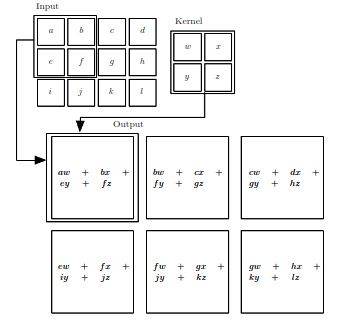
\includegraphics[width=0.45 \textwidth,keepaspectratio=true]{images/convolution.png}
 % convolution.png: 342x321 px, 72dpi, 12.06x11.32 cm, bb=0 0 342 321
 \caption{Abbildung zur Faltung \cite{CNNBook}}
 \label{fig:faltung}
\end{figure}
Mehrere dieser Kernel bilden zusammen ein Teil des Convolutional Layer. Dabei wird der Eingang des Layers wie in Abbildung \ref{fig:cnn} gezeigt auf jeden Kernel mittels der Faltung angewendet. Durch diese Faltung entstehen Erste Feature-Maps. Diese Feature-Maps werden im nächsten Schritt Komponentenweise als Eingabe für eine Aktivierungsfunktion benutzt. In Abbildung \ref{fig:cnn} wird ReLU als Aktivierungsfunktion benutzt\footnote{Für Erklärung Relu siehe \cite{neural}}. Um Overfitting zu vermeiden kann nach dem Anwenden der Aktivierungsfunktion eine Pooling Operation eingeführt werden. Pooling verkleinert die Größe der Feature-Map verkleinert.

Der Begriff Padding aus Abbildung \ref{fig:cnn} enthält einen Wert, der aussagt ob und wenn ja wieviele Pixel um das eigentlich Bild gelegt werden. Dies geschieht, um dem Kernel die Möglichkeit zu geben die Pixel am Rand des Bildes(bzw. der Featuremap der vorherigen Schicht) in mehreren Teilbildern zu verarbeiten.  

Beim Anwenden des Kernels auf die Eingabe kann jedes Teilbild oder weniger Teilbilder verwendet werden. Dies wird über den Parameter Stride kommuniziert. Beim Stride von Eins wird jedes Teilbild verwendet. Wird der Stride auf 2 gesetzt, so wird nach jedem verwendetem Teilbild eines ausgesetzt.


In einem CNN werden mehrere dieser Convolutional Layer hintereinander geschaltet, um komplexe Features erkennen zu können. 
\begin{figure}[H]
  \centering
  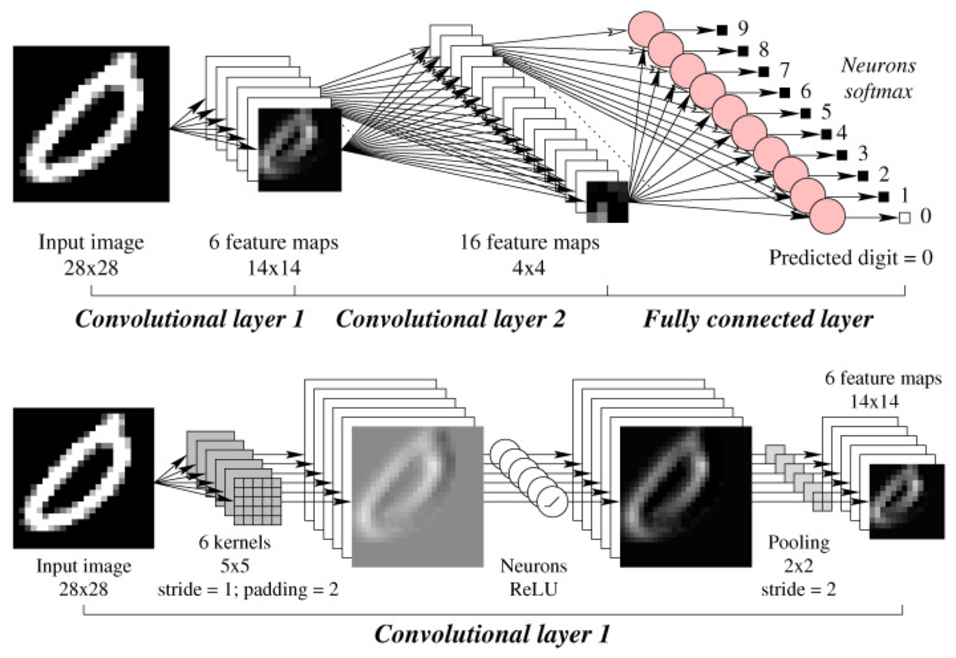
\includegraphics[width=0.75\textwidth]{images/cnn.pdf}
  \caption{Convolutional Neural Net \cite{CNNImg}}
  \label{fig:cnn}
\end{figure}



Eine beispielhafte Übersicht über die CNN-Architektur ist in Abbildung \ref{fig:cnn} zu sehen.

Die Fully-Connected-Layer errechnen aus den Ausgängen der Convolutional-Layer, in welche Klasse ein Objekt klassifiziert werden soll.  

Die Filter, die auf die Feature Maps bzw. die Eingabebilder angewendet werden, sind trainierbar. Zusätzlich sind auch die Gewichtungen des Fully-Connected Layers trainierbar. Das heißt durch den Trainingsprozess wird versucht die Werte in der Filtermatrix und des Fully-Connected Layer so zu verändern, dass das gesamte CNN besser klassifizieren kann. Für diese Veränderung wird ein Gradientenabstiegsverfahren, welches rückwärts durch die Schichten propagiert wird, benutzt.



\section{Überblick über die bisherigen wissenschaftlichen Methoden}
In diesem Unterkapitel wird ein Überblick über die bisher erforschten Methoden des schnelleren Trainieren und desEffizienten Architekturverbesserns gegeben. In Paragraph \ref{sec:fp16} wird die Verwendung von anderen Zahlenformaten zur Zeiteinsparung beim Training gegeben. In Paragraph xxx wird erläutert, wie sich das Gradientenabstiegsverfahren beschleunigen lässt. 
